\documentclass[12pt]{article}
\usepackage[margin=0.5in]{geometry}
\usepackage{multirow}
\usepackage{graphicx} 
\usepackage{caption}
\usepackage{subcaption}

\begin{document}

\section*{The 17 Plane Groups}

\begin{figure}[htp]
 \centering
    \begin{subfigure}[b]{0.45\textwidth}
        \centering
        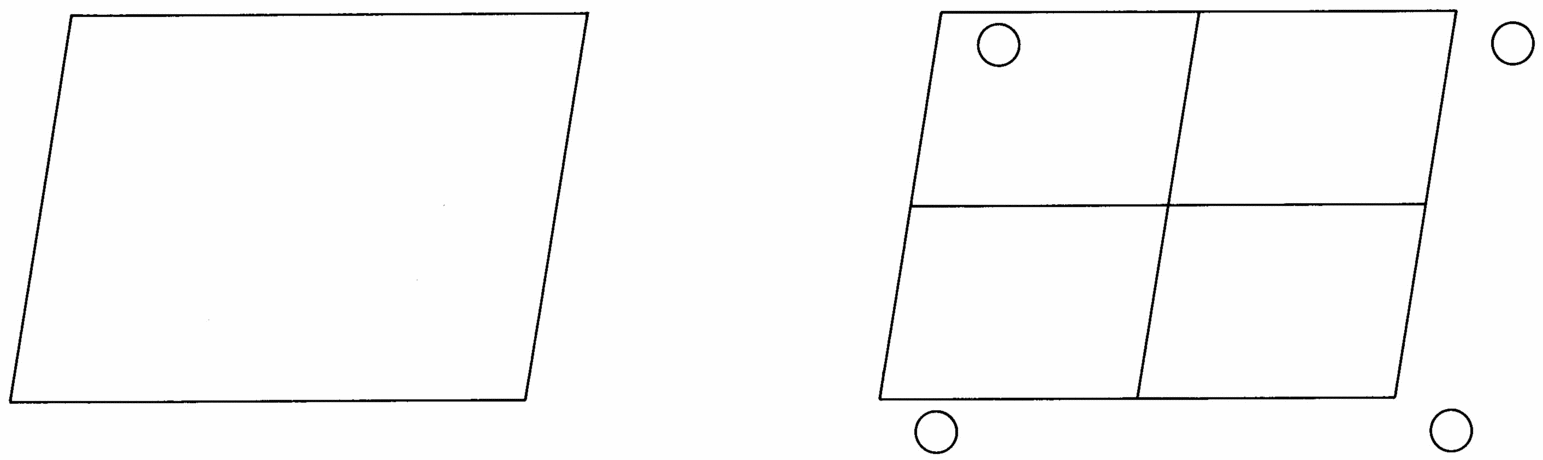
\includegraphics[width=\textwidth]{planegroups/1.png}
        \caption*{p1}
    \end{subfigure}
    ~
    \begin{subfigure}[b]{0.45\textwidth}
        \centering
        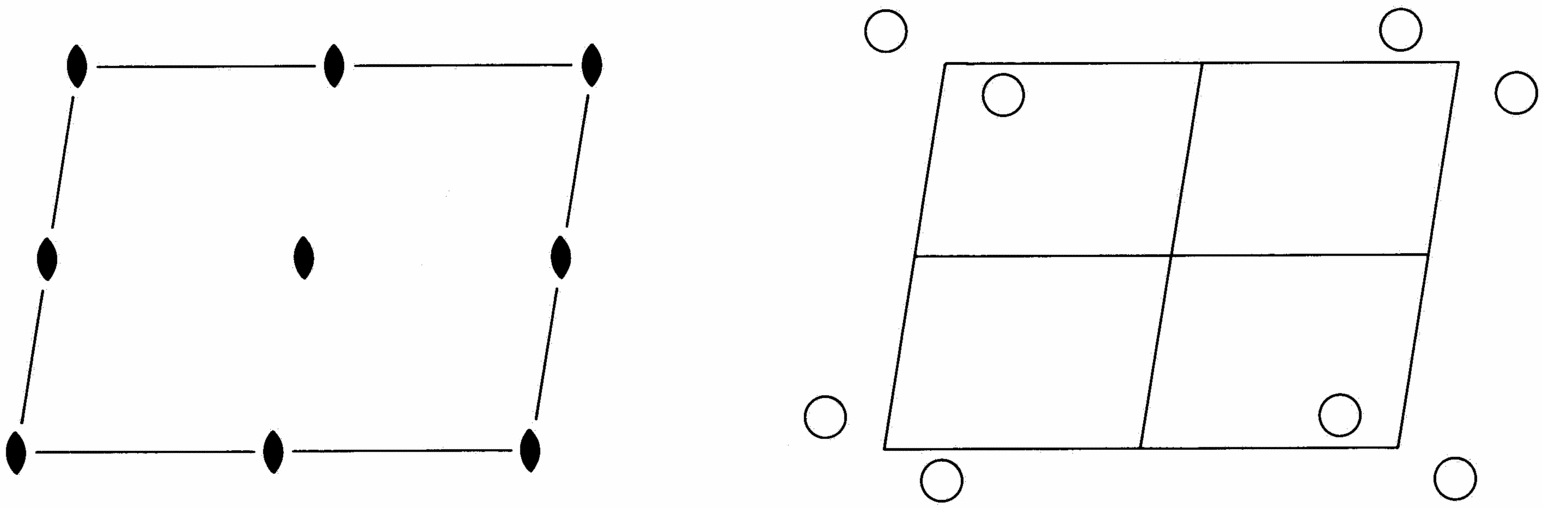
\includegraphics[width=\textwidth]{planegroups/2.png}
        \caption*{p2}
    \end{subfigure}
    \begin{subfigure}[b]{0.45\textwidth}
        \centering
        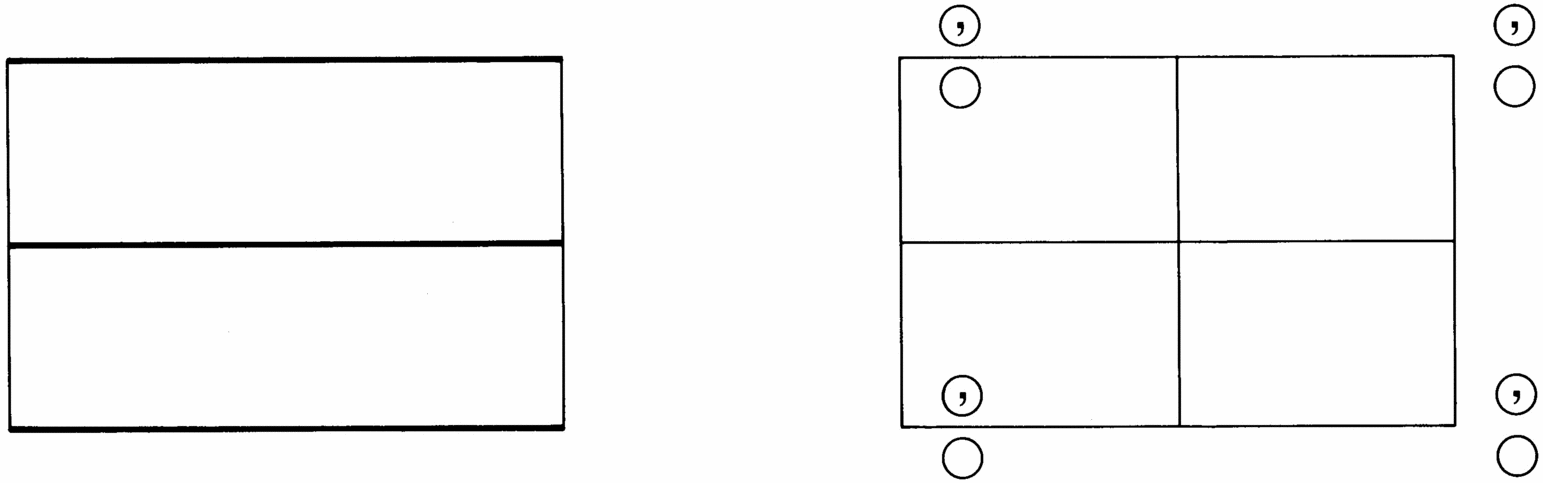
\includegraphics[width=\textwidth]{planegroups/3.png}
        \caption*{pm}
    \end{subfigure}
	~    
    \begin{subfigure}[b]{0.45\textwidth}
        \centering
        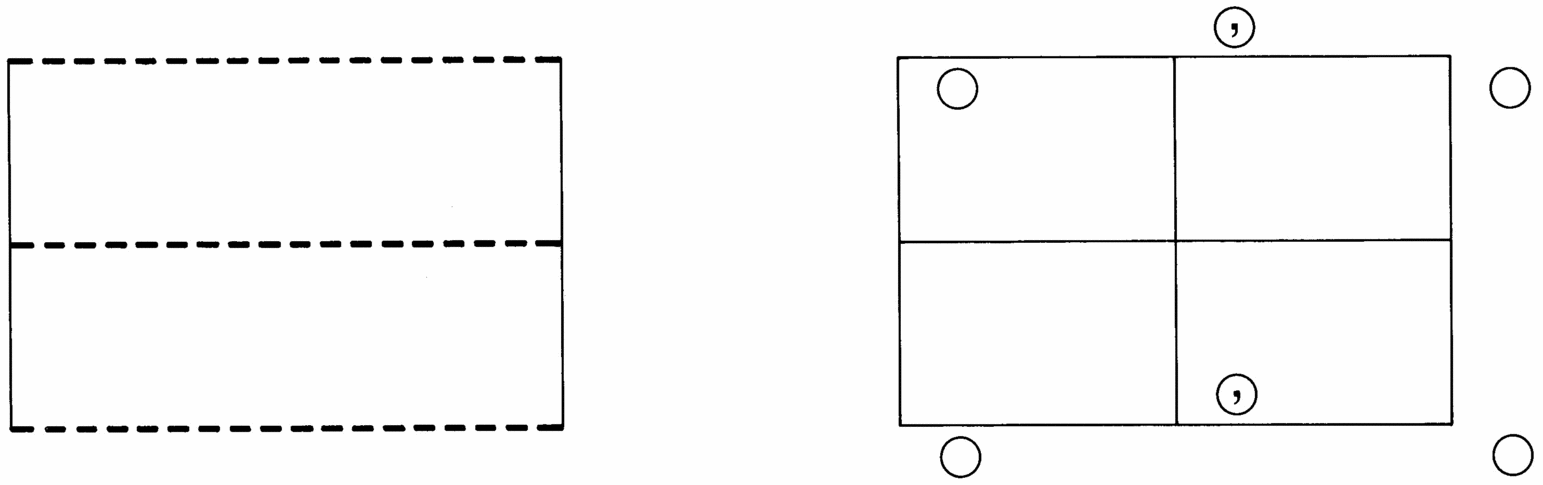
\includegraphics[width=\textwidth]{planegroups/4.png}
        \caption*{pg}
    \end{subfigure}
    \begin{subfigure}[b]{0.45\textwidth}
        \centering
        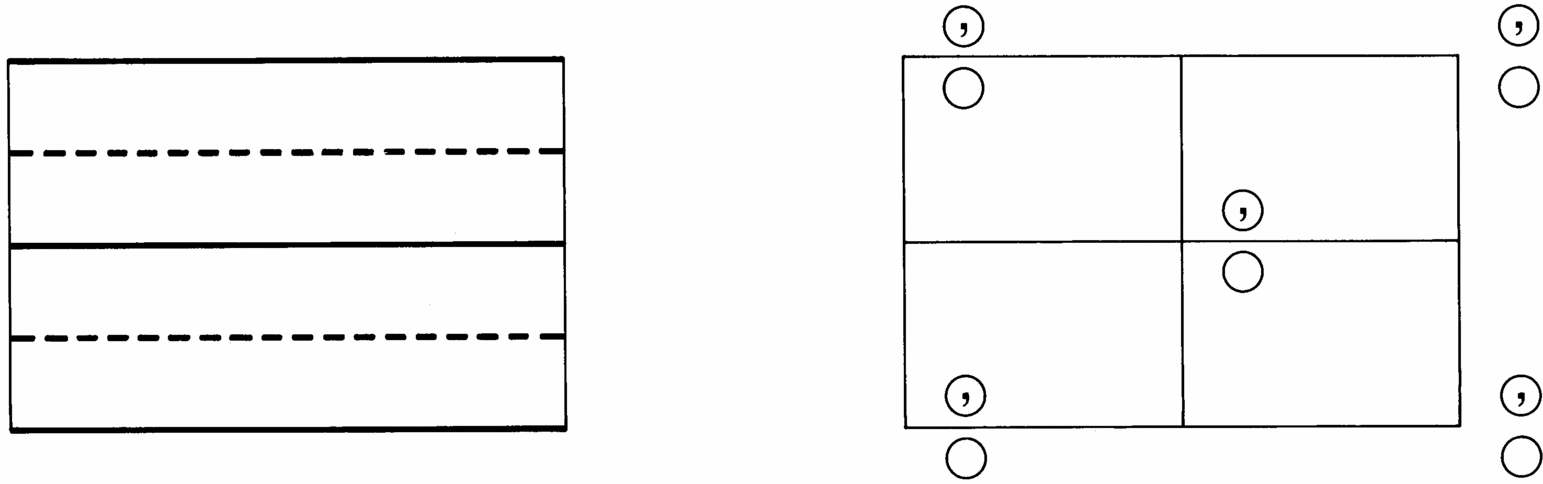
\includegraphics[width=\textwidth]{planegroups/5.png}
        \caption*{cm}
    \end{subfigure}
	~    
    \begin{subfigure}[b]{0.45\textwidth}
        \centering
        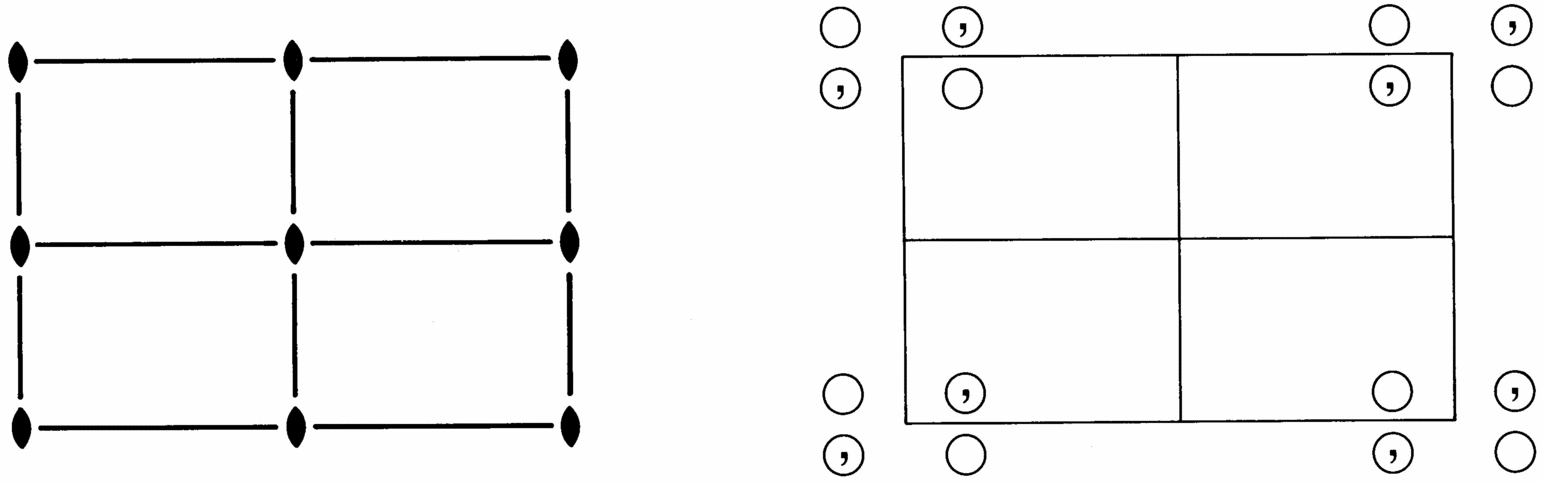
\includegraphics[width=\textwidth]{planegroups/6.png}
        \caption*{p2mm}
    \end{subfigure}
    \begin{subfigure}[b]{0.45\textwidth}
        \centering
        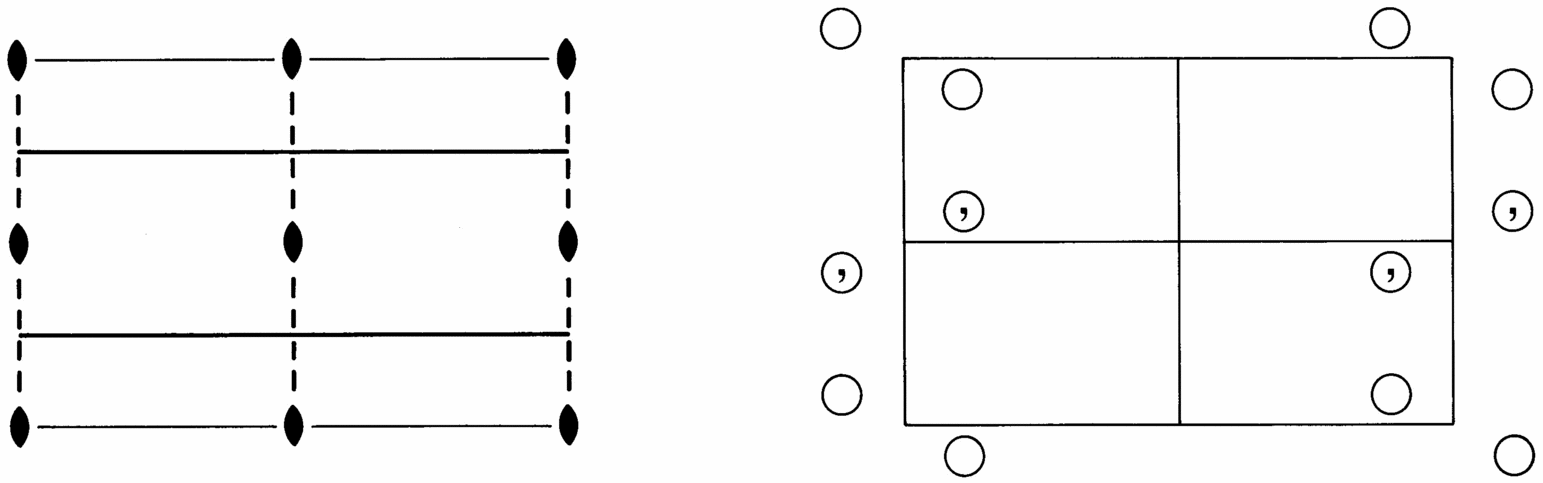
\includegraphics[width=\textwidth]{planegroups/7.png}
        \caption*{p2mg}
    \end{subfigure}
	~    
    \begin{subfigure}[b]{0.45\textwidth}
        \centering
        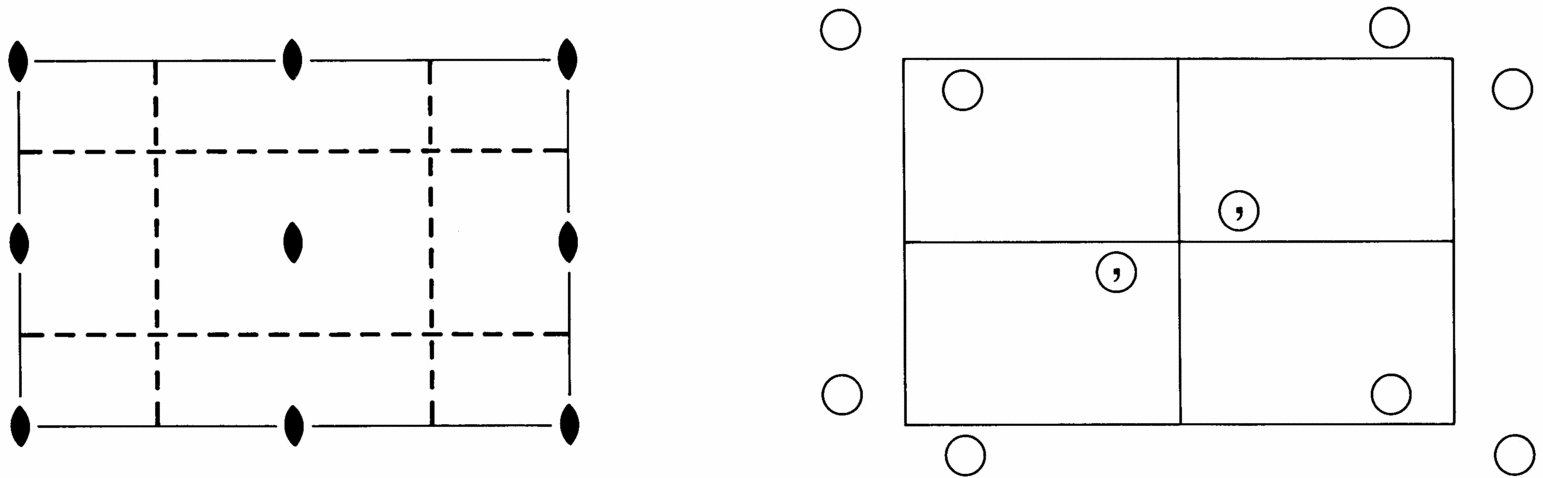
\includegraphics[width=\textwidth]{planegroups/8.png}
        \caption*{p2gg}
    \end{subfigure}
    \begin{subfigure}[b]{0.45\textwidth}
        \centering
        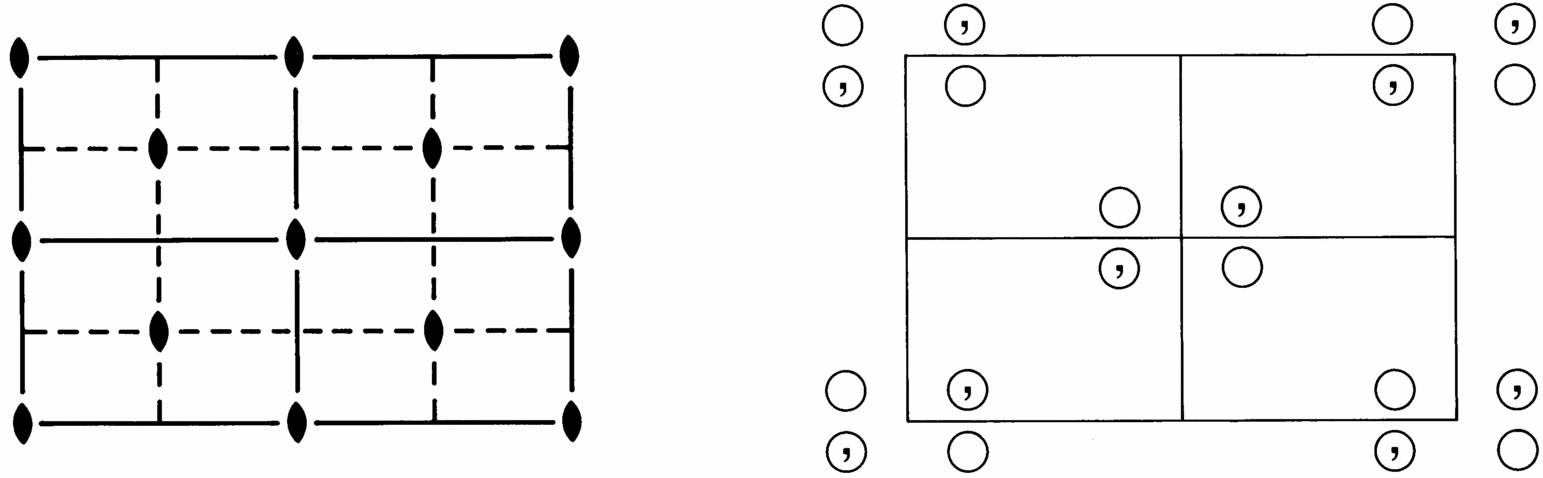
\includegraphics[width=\textwidth]{planegroups/9.png}
        \caption*{c2mm}
    \end{subfigure}
	~    
    
\end{figure}

\begin{figure}
 \centering
    \begin{subfigure}[b]{0.45\textwidth}
        \centering
        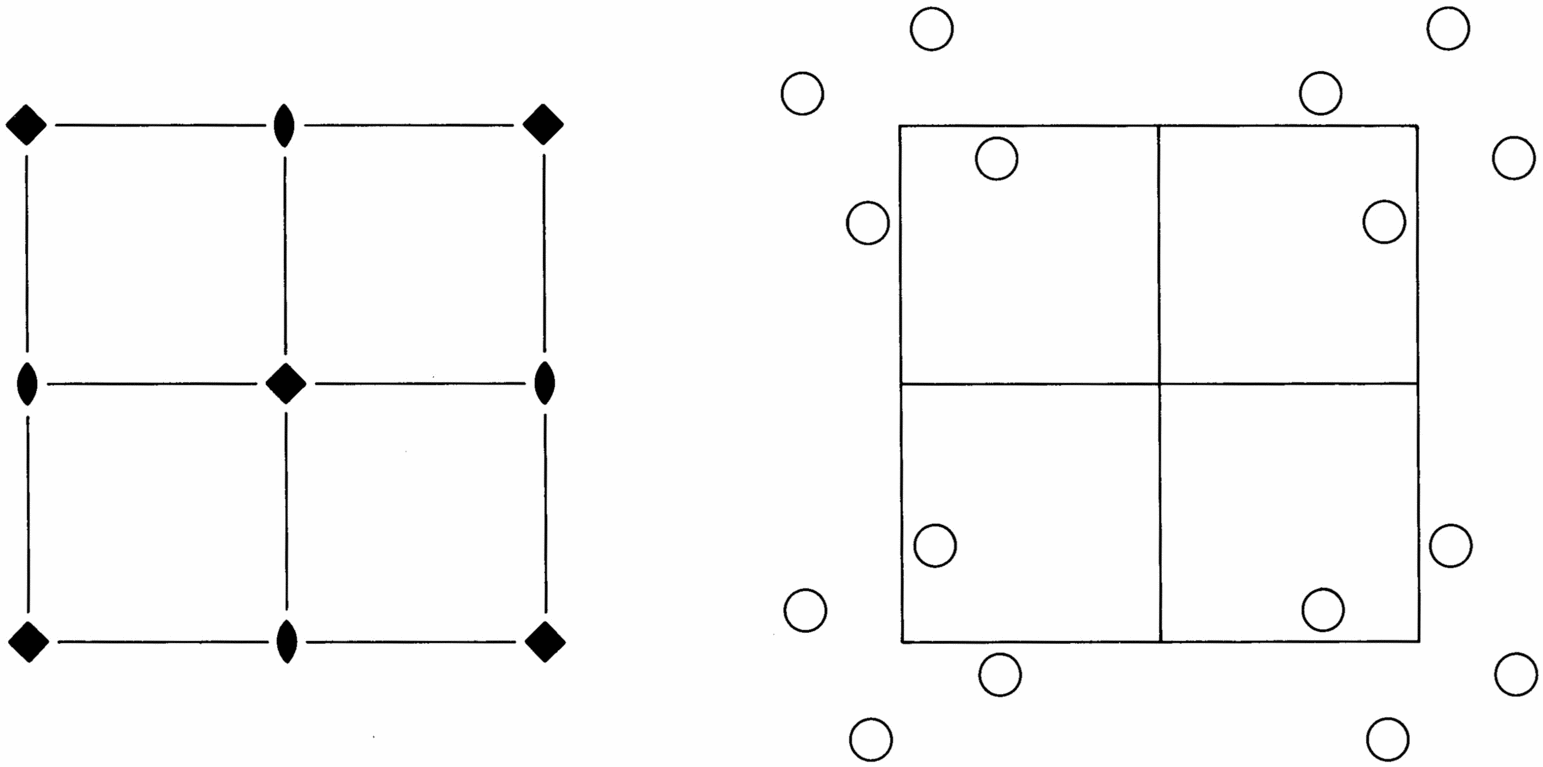
\includegraphics[width=\textwidth]{planegroups/10.png}
        \caption*{p4}
    \end{subfigure}
    ~
    \begin{subfigure}[b]{0.45\textwidth}
        \centering
        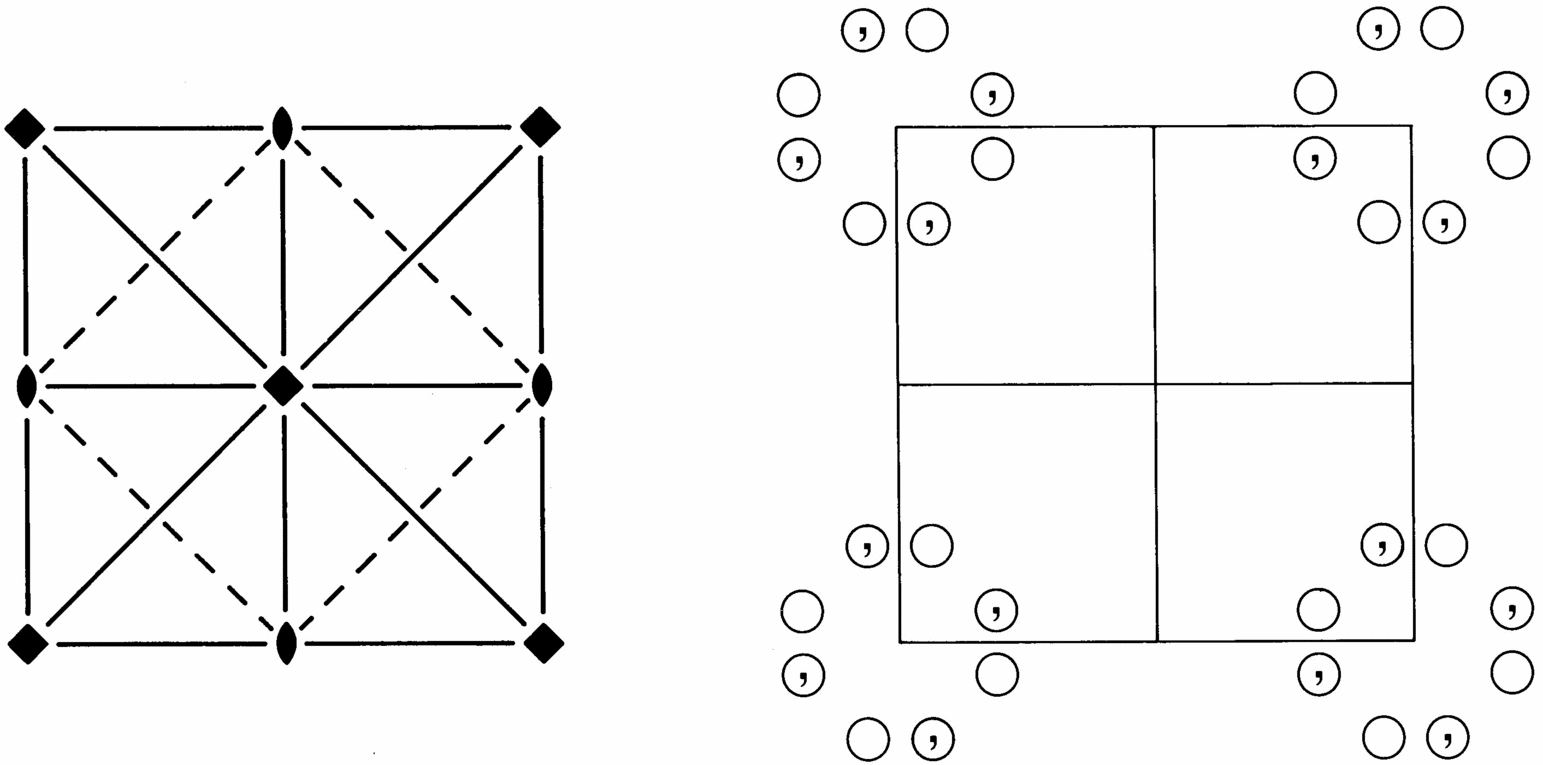
\includegraphics[width=\textwidth]{planegroups/11.png}
        \caption*{p4mm}
    \end{subfigure}
	\begin{subfigure}[b]{0.5\textwidth}
        \centering
        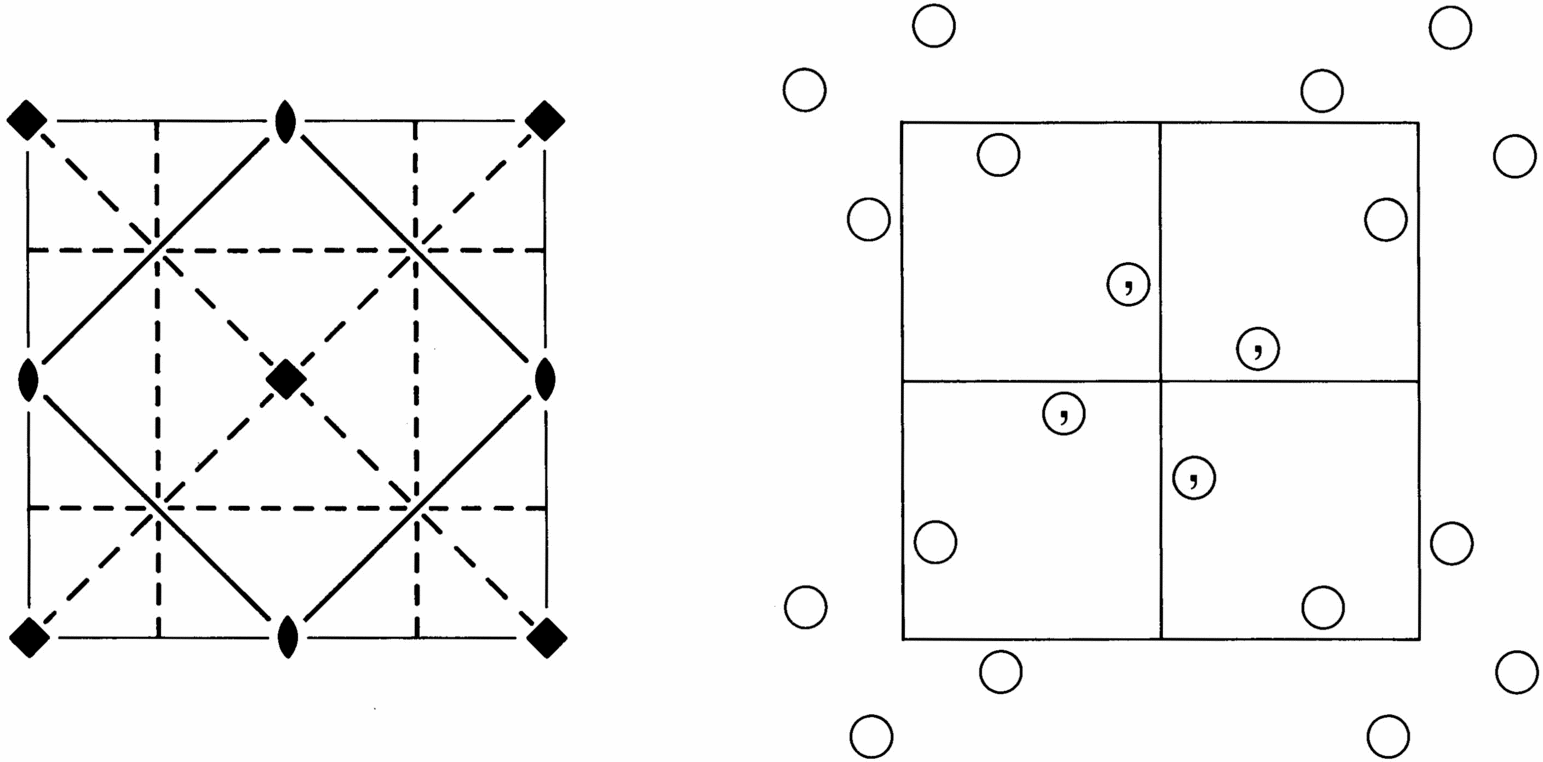
\includegraphics[width=\textwidth]{planegroups/12.png}
        \caption*{p4gm}
    \end{subfigure}\\    
    \begin{subfigure}[b]{0.45\textwidth}
        \centering
        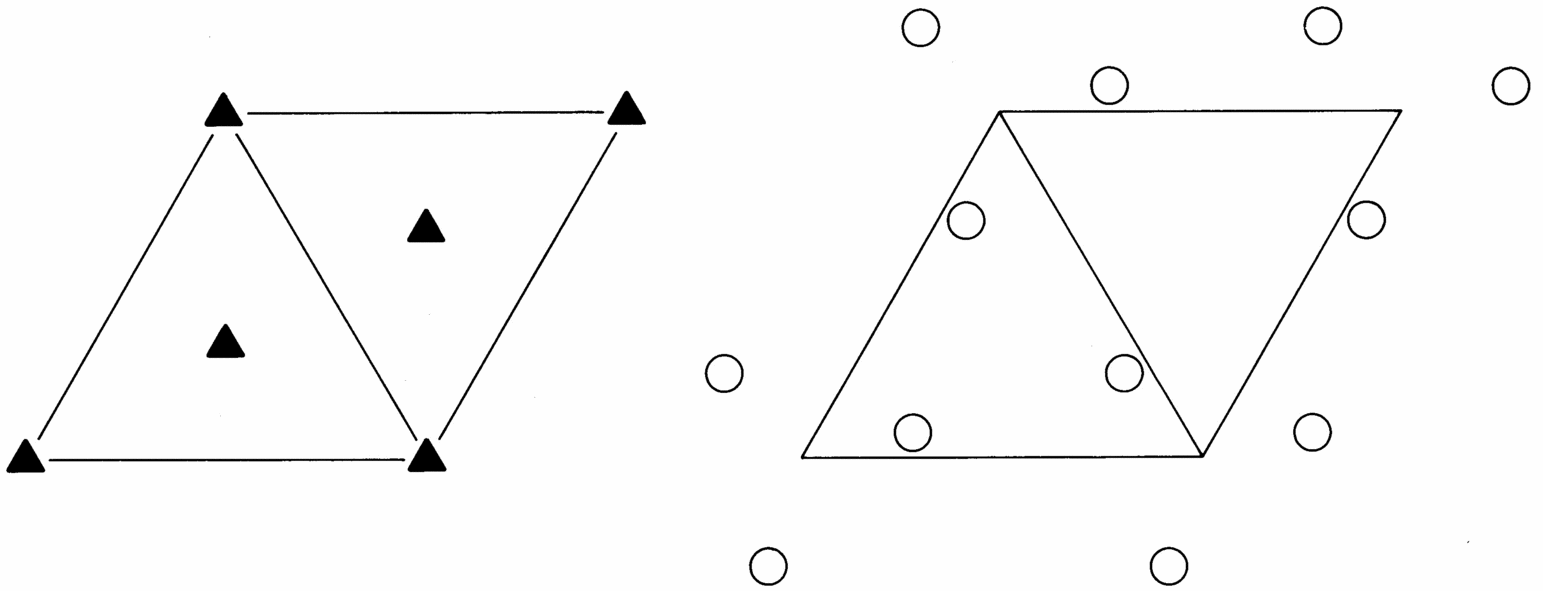
\includegraphics[width=\textwidth]{planegroups/13.png}
        \caption*{p3}
    \end{subfigure}
    ~
    \begin{subfigure}[b]{0.45\textwidth}
        \centering
        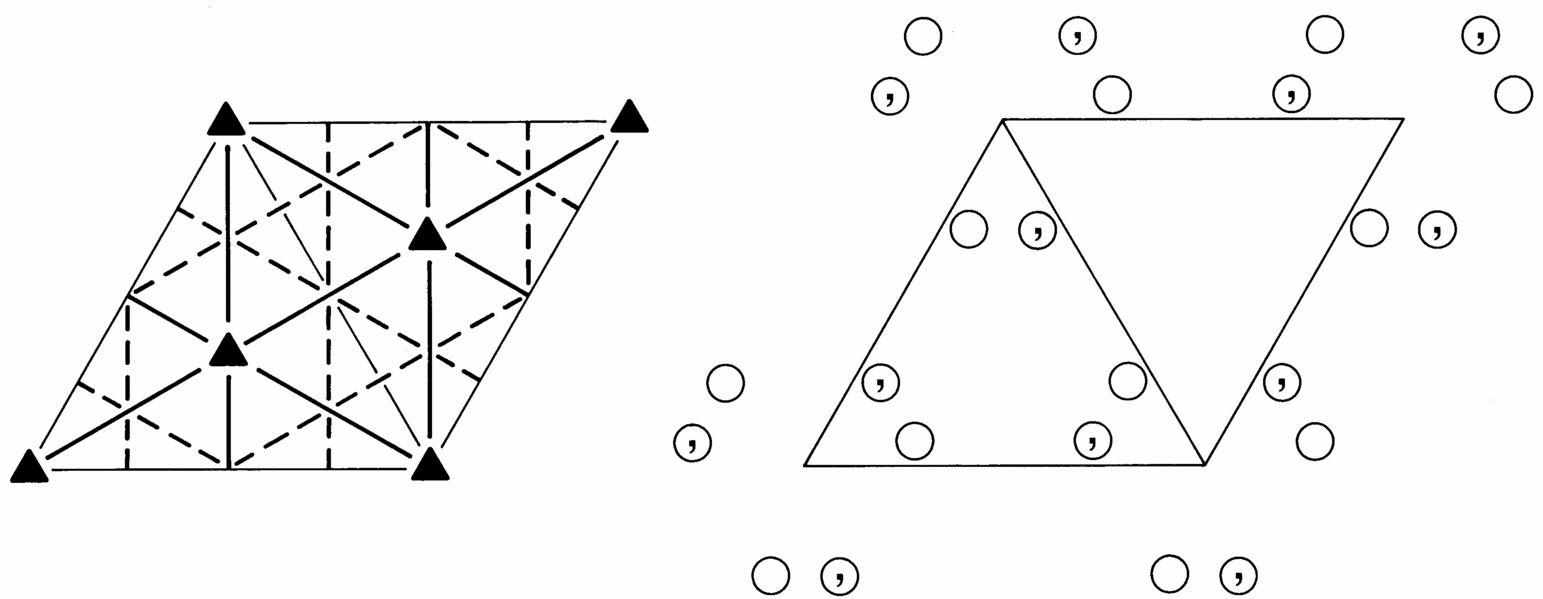
\includegraphics[width=\textwidth]{planegroups/14.png}
        \caption*{p3m1}
    \end{subfigure}
    \begin{subfigure}[b]{0.45\textwidth}
        \centering
        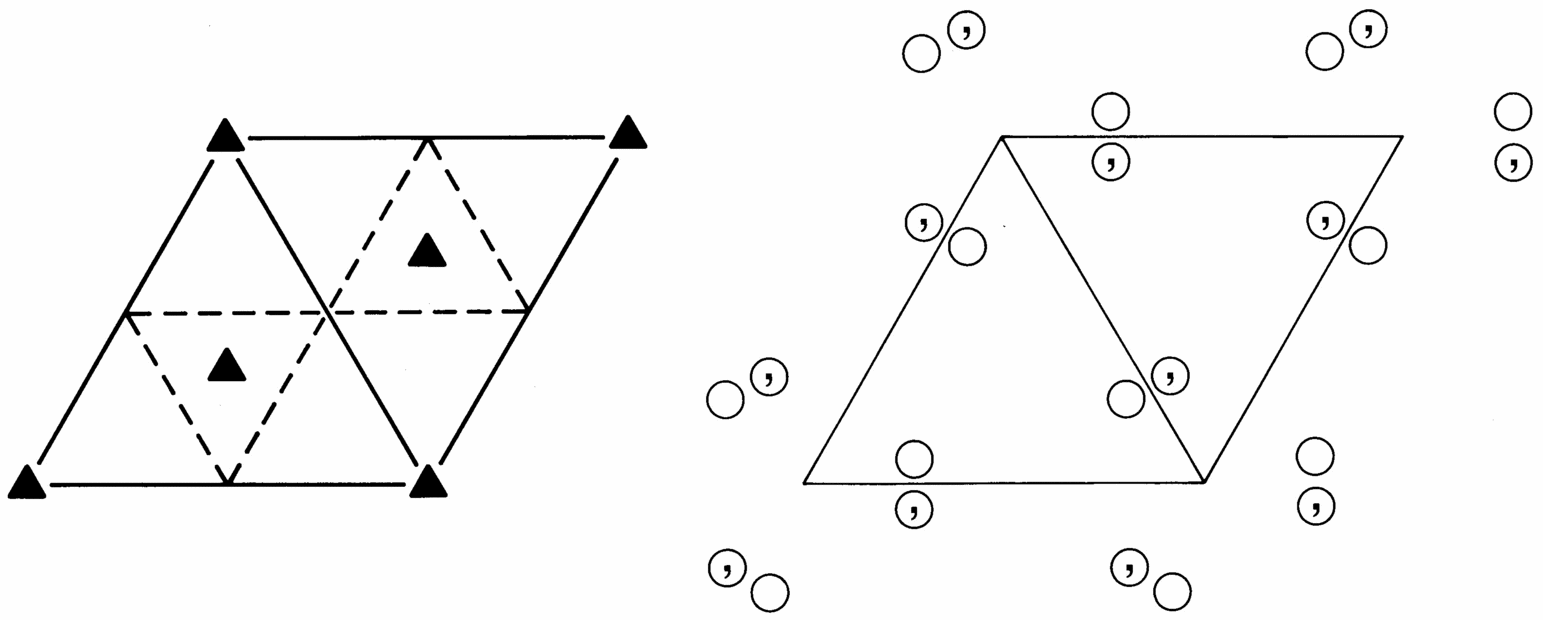
\includegraphics[width=\textwidth]{planegroups/15.png}
        \caption*{p31m}
    \end{subfigure}\\
    \begin{subfigure}[b]{0.45\textwidth}
        \centering
        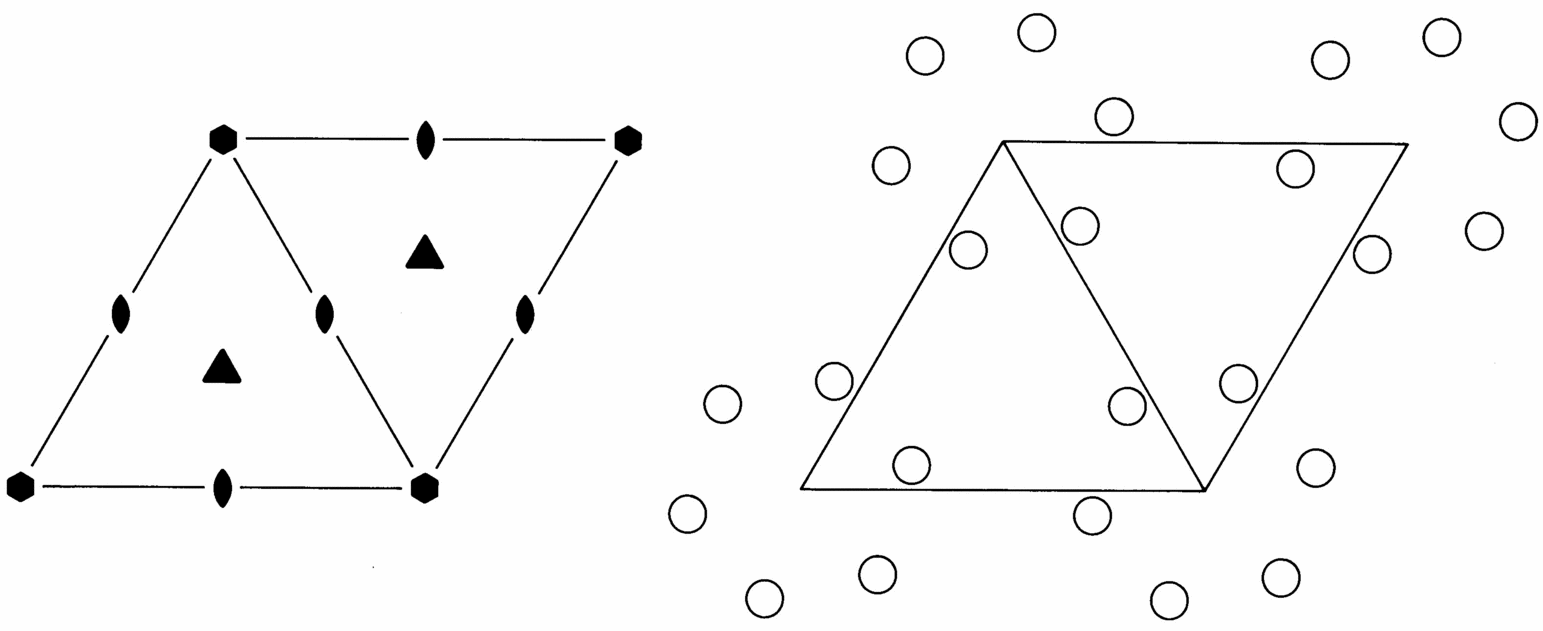
\includegraphics[width=\textwidth]{planegroups/16.png}
        \caption*{p6}
    \end{subfigure}
    \begin{subfigure}[b]{0.45\textwidth}
        \centering
        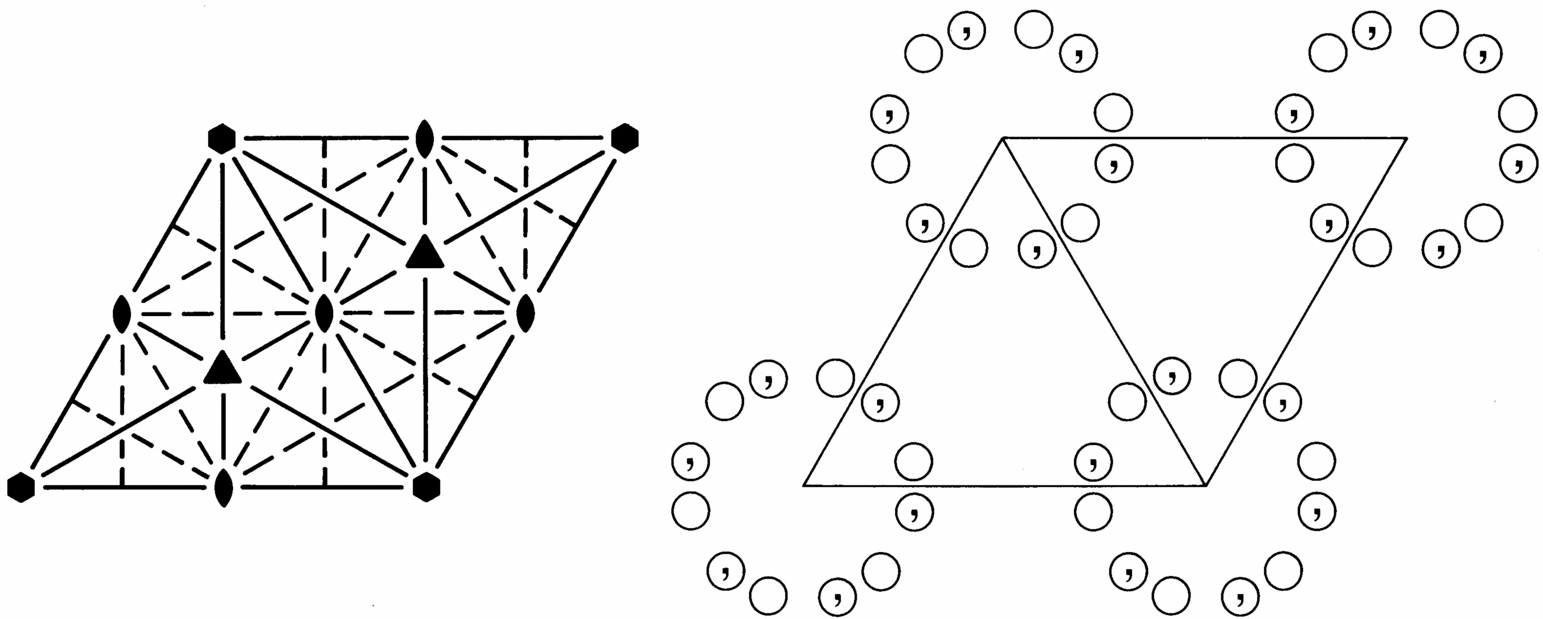
\includegraphics[width=\textwidth]{planegroups/17.png}
        \caption*{p6mm}
    \end{subfigure}
\end{figure}

\end{document}
%
% ****** End of file apstemplate.tex ******
